%%%%%%%%%%%%%%%%%%%%%%%%%%%%%%%%%%%%%%%%%%%%%%%%%%%%%%%%%%%%%%%%%%%%%%%%%%%%%%%
% \subsection{Introduction}
%%%%%%%%%%%%%%%%%%%%%%%%%%%%%%%%%%%%%%%%%%%%%%%%%%%%%%%%%%%%%%%%%%%%%%%%%%%%%%%
% \begin{frame}
%  \begin{colorblock}{blue}{lightblue}{ }
%     \Large \textbf{Introduction}
%   \end{colorblock}
% \end{frame}

\begin{frame}
\frametitle{Overview of the Lecture}
\begin{itemize}
	\item {\bf General overview of cluster scheduling principles}
	\begin{itemize}
		\item General objectives
		\item A taxonomy
		\item Current architectures
	\end{itemize}

\vspace{20pt}
	
	\item {\bf In depth presentation of three representative examples}
	\begin{itemize}
		\item Yarn
		\item Mesos
		\item Borg (Kubernetes)
	\end{itemize}
\end{itemize}
\end{frame}

%%%%%%%%%%%%%%%%%%%%%%%%%%%%%%%%%%%%%%%%%%%%%%%%%%%%%%%%%%%%%%%%%%%%%%%%%%%%%%%
\subsection{Cluster Scheduling Principles}
%%%%%%%%%%%%%%%%%%%%%%%%%%%%%%%%%%%%%%%%%%%%%%%%%%%%%%%%%%%%%%%%%%%%%%%%%%%%%%%
\begin{frame}
 \begin{colorblock}{blue}{lightblue}{ }
    \Large \textbf{Cluster Scheduling Principles}
  \end{colorblock}
\end{frame}

\begin{frame}\frametitle{Objectives}
\begin{itemize}
	\item {\bf Large-scale clusters are expensive, so it is important to use them well}
	\begin{itemize}
		\item Cluster utilization and efficiency are key indicators for good resource management and scheduling decisions
		\item Translates directly to cost arguments: better scheduling $\to$ smaller clusters
	\end{itemize}

\vspace{10pt}

	\item {\bf Multiplexing to the rescue}
	\begin{itemize}
		\item Multiple, heterogeneous mixes of application run conccurently
		\item[$\to$] The scheduling problem is a challenge
	\end{itemize}

\vspace{10pt}

	\item {\bf Scalability bottlenecks}
	\begin{itemize}
		\item Cluster and workload sizes keep growing
		\item Scheduling complexity roughly proportional to cluster size
		\item[$\to$] Schedulers must be scalable
	\end{itemize}
\end{itemize}
\end{frame}

\begin{frame}\frametitle{Current Scheduler Architectures}
\begin{figure}[h]
  \centering
  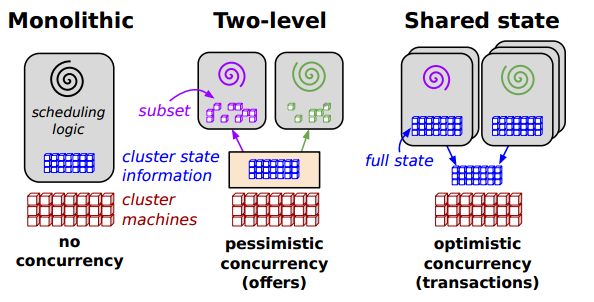
\includegraphics[scale=0.3]{./figures/intro_arch}
  \label{fig:intro_arch}
\end{figure}
\begin{itemize}
	\item {\bf Monolitic:} use a centralized scheduling and resource management algorithm for all jobs
	\begin{itemize}
		\item Difficult to add new scheduling policies
		\item Do not scale well to large cluster sizes
	\end{itemize}
	
\vspace{10pt}

	\item {\bf Two-level:} single resource manager that grants resources to independent ``framework schedulers''
	\begin{itemize}
		\item Flexibility in accommodating multiple application frameworks
		\item Resource management and locking are conservative, which can hurt cluster utilization and performance
	\end{itemize}
\end{itemize}
\end{frame}

\begin{frame}\frametitle{Typical workloads to support}
\begin{itemize}
	\item {\bf Cluster scheduler must support heterogeneous workloads and clusters}
	\begin{itemize}
		\item Clusters are made of several generations of machines
		\item Workloads evolve in time, and can be made of a variety of applications
	\end{itemize}

\vspace{10pt}

	\item {\bf Rough categorization of job types}
	\begin{itemize}
		\item Batch jobs: e.g., MapReduce computations
		\item Service jobs: e.g., end-user facing web service
	\end{itemize}

\vspace{10pt}

	\item {\bf Knowing your workload is fundamental!}
	\begin{itemize}
		\item Next, some examples from real cluster traces
		\item The rationale: measurements can inform scheduling design
	\end{itemize}
\end{itemize}
\end{frame}

\begin{frame}\frametitle{Real cluster trace: workload characteristics}
\begin{figure}[h]
  \centering
  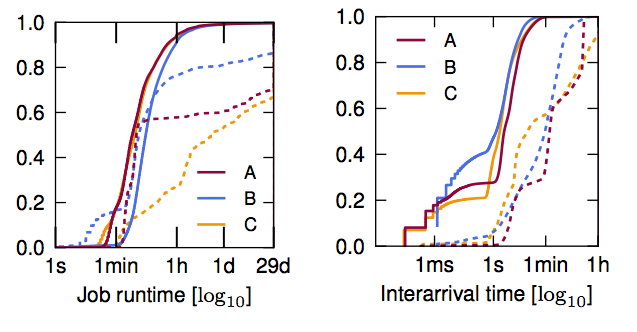
\includegraphics[scale=0.4]{./figures/intro_trace1}
  \label{fig:intro_trace1}
\end{figure}
\begin{itemize}
	\item Solid lines: batch jobs, dashed lines: service jobs
\end{itemize}
\end{frame}

\begin{frame}\frametitle{Real cluster trace: workload characteristics}
\begin{figure}[h]
  \centering
  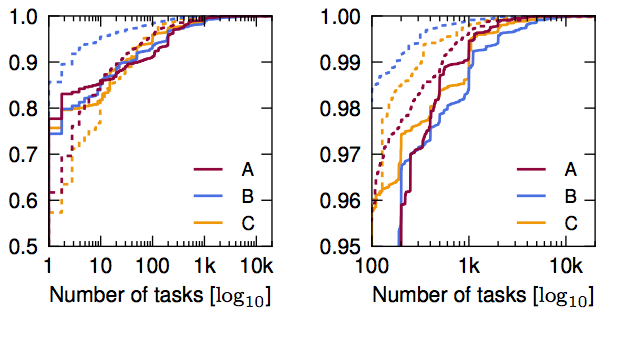
\includegraphics[scale=0.4]{./figures/intro_trace2}
  \label{fig:intro_trace2}
\end{figure}
\begin{itemize}
	\item Solid lines: batch jobs, dashed lines: service jobs
\end{itemize}
\end{frame}

\begin{frame}\frametitle{Short Taxonomy of Scheduling Design Issues}
\begin{itemize}
	\item {\bf Scheduling Work Partitioning:} how to distribute work across frameworks
	\begin{itemize}
		\item Workload-oblivious load-balancing
		\item Workload partitioning and specialized schdulers
		\item Hybrid
	\end{itemize}

\vspace{20pt}

	\item {\bf Resource choice:} which cluster resources are available to concurrent frameworks
	\begin{itemize}
		\item All resources available
		\item A subset of cluster resources is granted (or offered)
		\item NOTE: preemption primitives help scheduling flexibility at the cost of potentially wasting work
	\end{itemize}
\end{itemize}
\end{frame}

\begin{frame}\frametitle{Short Taxonomy of Scheduling Design Issues}
\begin{itemize}
	\item {\bf Interference:} what to do when multiple frameworks attempt at using the same resources
	\begin{itemize}
		\item Pessimistic concurrency control: make sure to avoid conflicts, by partitionning resources across frameworks
		\item Optimistic concurrency control: hope for the best, otherwise detect and undo conflicting claims
	\end{itemize}

\vspace{20pt}

	\item {\bf Allocation Granularity: } task ``scheduling'' policies
	\begin{itemize}
		\item Atomic, all-or-nothing gang scheduling: e.g. MPI
		\item Incremental placement, hoarding: e.g. MapReduce
	\end{itemize}

\vspace{20pt}

	\item {\bf Cluster-wide behavior: } some requirements need global view
	\begin{itemize}
		\item Fairness across frameworks
		\item Global notion of priority
	\end{itemize}
\end{itemize}
\end{frame}

\begin{frame}\frametitle{Summary of design knobs}
\begin{figure}[h]
  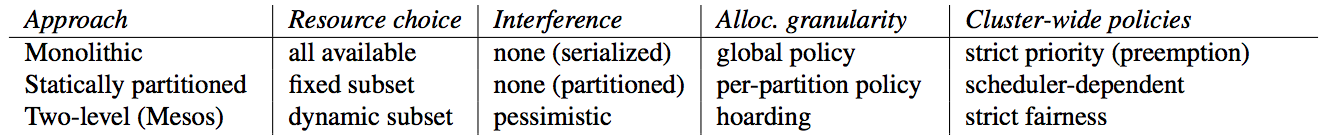
\includegraphics[scale=0.28]{./figures/intro_design}
  \label{fig:intro_design}
\end{figure}
\begin{itemize}
	\item {\bf Comparison of cluster scheduling approaches}
\end{itemize}
\end{frame}

\begin{frame}\frametitle{Architecture Details}
\begin{itemize}
	\item {\bf High-level summary of scheduling objectives}
	\begin{itemize}
		\item Minimize the job queueing time, or more generally, the system response time (queueing + service times)
		\item Subject to
		\begin{itemize}
			\item Priorities among jobs
			\item Per-job constraints
			\item Failure tolerance
			\item Scalability
		\end{itemize}
	\end{itemize}

\vspace{20pt}

	\item {\bf Scheduling architectures}
	\begin{itemize}
		\item Monolithic schedulers
		\item Statically partitioned schedulers
		\item Two-level schedulers
		\item Shared-state schedulers (cf. Omega paper)
	\end{itemize}
\end{itemize}
\end{frame}

\begin{frame}\frametitle{Monolithic Schedulers}
\begin{itemize}
	\item {\bf Single centralized instance}
	\begin{itemize}
		\item Typical of HPC setting
		\item Implements all policies in a single code base
		\item Applies the same scheduling algorithm to all incoming jobs
	\end{itemize}

\vspace{20pt}

	\item {\bf Alternative designs}
	\begin{itemize}
		\item Support multiple code paths for different jobs
		\item Each path implements a different scheduling logic
		\item[$\to$] Difficult to implement and maintain
	\end{itemize}
\end{itemize}
\end{frame}

\begin{frame}\frametitle{Statically Partitioned Schedulers}
\begin{itemize}
	\item {\bf Standard ``Cloud-computing'' approach}
	\begin{itemize}
		\item Underlying assumption: each framework has complete control over a set of resources
		\item Depend on statically partitioned, dedicated resources
		\item Examples: Hadoop 1.0, Quincy scheduler
	\end{itemize}

\vspace{20pt}

	\item {\bf Problems with static partitioning}
	\begin{itemize}
		\item Fragmentation of resources
		\item Sub-optimal cluster utilization
	\end{itemize}
\end{itemize}
\end{frame}

\begin{frame}\frametitle{Two-level Schedulers}
\begin{itemize}
	\item {\bf Obviates the problems of static partitioning}
	\begin{itemize}
		\item Dynamic allocation of resources to concurrent frameworks
		\item Use a ``logically centralized'' coordinator to decide how many resources to grant
	\end{itemize}
	\item {\bf A first example: Mesos}
	\begin{itemize}
		\item Centralized resource allocator, with dynamic cluster partitioning
		\item {\bf Available} resources are {\it offered} to competing frameworks
		\item Avoids interference by exclusive offers
		\item Frameworks lock resources by accepting offers $\to$ {\bf pessimistic concurrency control}
		\item No global cluster state available to frameworks
	\end{itemize}
	\item {\bf Another tricky example: YARN}
	\begin{itemize}
		\item Centralized resource allocator (RM), with per-job framework master (AM)
		\item AM only provides job management services, not proper scheduling
		\item[$\to$] YARN is closer to a monolithic architecture
	\end{itemize}
\end{itemize}
\end{frame}

